\chapter{Licht und Farben}
\Defi (sichtbares) \textbf{Licht} sind elektromagnetische Wellen verschiedener Wellenlänge (ca. zwischen 400--700 nm)
	Die Wellenlänge $\lambda$ entscheidet über die \textbf{Farbe}. Das meiste Licht ist eine Mischung von verschiedenen Wellenlängen.
% 5.2
\begin{center}
 
\includegraphics[height=3cm]{Prism_rainbow_schema.eps}
 % http://commons.wikimedia.org/wiki/File:Prism_rainbow_schema.png
\end{center}
Wenn Licht auf einen Gegenstand trifft, dann wird es in unterschiedlichem Maß zurückgeworfen, je nach Wellenlänge
 %5.3
Wenn Licht einen filter durchdringt, ist es analog (subtraktive Farbmischung).

\section{Farbensehen im menschlichen Auge}
Es gibt drei Arten von lichtempfindlichen \emph{Zapfen} (R, G, B)
\begin{center}
\begin{pspicture}(0,0)(6,3.3)
\rput[bl](0,0){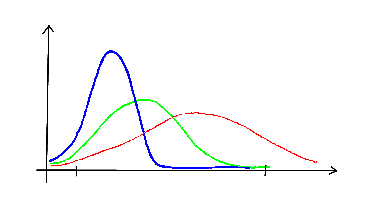
\includegraphics{zapfen.eps}}
\rput[t](1,0.3){400}
\rput[t](4.167,0.3){700}
\rput[t](5.5,0.5){$\lambda$}
\rput[bl](0.2,3){Empfindlichkeit -- $e_R(\lambda), e_G(\lambda), e_B(\lambda)$}
\end{pspicture}
\end{center}
Erregung der "`roten"' Zapfen bei einer Lichtquelle mit Intensitätsfunktion $f(\lambda)$
\[r = \int f(\lambda) \cdot e_R(\lambda)\ \mathrm{d} y \qquad f(\lambda)\]
analog "`grün"': $g = \int f(\lambda) \cdot e_G(\lambda)\ \mathrm{d} y$\\
analog "`blau"': $b = \int f(\lambda) \cdot e_B(\lambda)\ \mathrm{d} y$
\begin{itemize}
 \item Verschiedene Lichtquellen mit verschiednen spektraler Zusammensetzung erzeugen den gleichen Farbeindruck, wenn 	sie die gleichen $(r,g,b)$-Werte hervorbringen.
 \item Dreidimensionaler Farbraum, aber nicht alle $(r,g,b)$-Werte erreichbar\\
	(Wenn $g > 0 \Rightarrow r > 0$ oder $b > 0$, $(r,g,b) = (0,1,0)$ gibt es nicht)
 \item Wenn man $f(\lambda)$ mit einem Skalar $c > 0$ multipliziert, dann ändert sich nur die Helligkeit, nicht die
	Farbe. Entsprechend wird $(r,g,b)$ mit einem Skalar multipliziert.
 \item Normalisierung auf $r+b+g=1$ führt auf einen zweidimensionalen Farbraum, bei dem die Helligkeit konstant ist.
\end{itemize}
In der Computergrafik tut man so, als ob es nur \emph{drei} verschiedene Wellenlängen (Grundfarben) gibt: {\color{red}R}ot, {\color{green}G}rün und {\color{blue}B}lau
\begin{center}
\begin{pspicture}(0.5,0.5)(4,3)
	\psline[linecolor=red]{-*}(1,0)(1,2)\uput{2pt}[-90](1,0){\color{red}R}
	\psline[linecolor=green]{-*}(2,0)(2,2)\uput{2pt}[-90](2,0){\color{green}G}
	\psline[linecolor=blue]{-*}(3,0)(3,2)\uput{2pt}[-90](3,0){\color{blue}B}
	\psaxes[labels=none,ticks=none]{->}(0,0)(-0.1,-0.1)(4,2.5)
\end{pspicture}
\end{center}